\section{Fairness Snapshot}
To monitor distributional harms, we audit ranking quality across user cohorts and catalog attributes. The current snapshot focuses on NDCG@10 disparities; the observed parity gap is \parityGap{} when comparing the most and least served groups in Table~\ref{tab:parity}. Figure~\ref{fig:parity-fig} visualizes relative performance, guiding dataset rebalancing or post-processing mitigations when disparities widen.

\begin{table}[h]
    \centering
    \captionsetup{width=.9\linewidth}
    \caption{Group-wise NDCG@10 parity assessment.}
    \label{tab:parity}
    \IfFileExists{auto/parity_table.tex}{% Auto-generated parity table (fallback)
\begin{tabular}{ll}
\toprule
Group & NDCG@10 \
\midrule
N/A & N/A \
\bottomrule
\end{tabular}
}{\begin{tabular}{lll}\toprule Group & Value & Notes \\ \midrule N/A & N/A & Data unavailable \\ \bottomrule \end{tabular}}
\end{table}

\begin{figure}[h]
    \centering
    \IfFileExists{parity_language_bar.png}{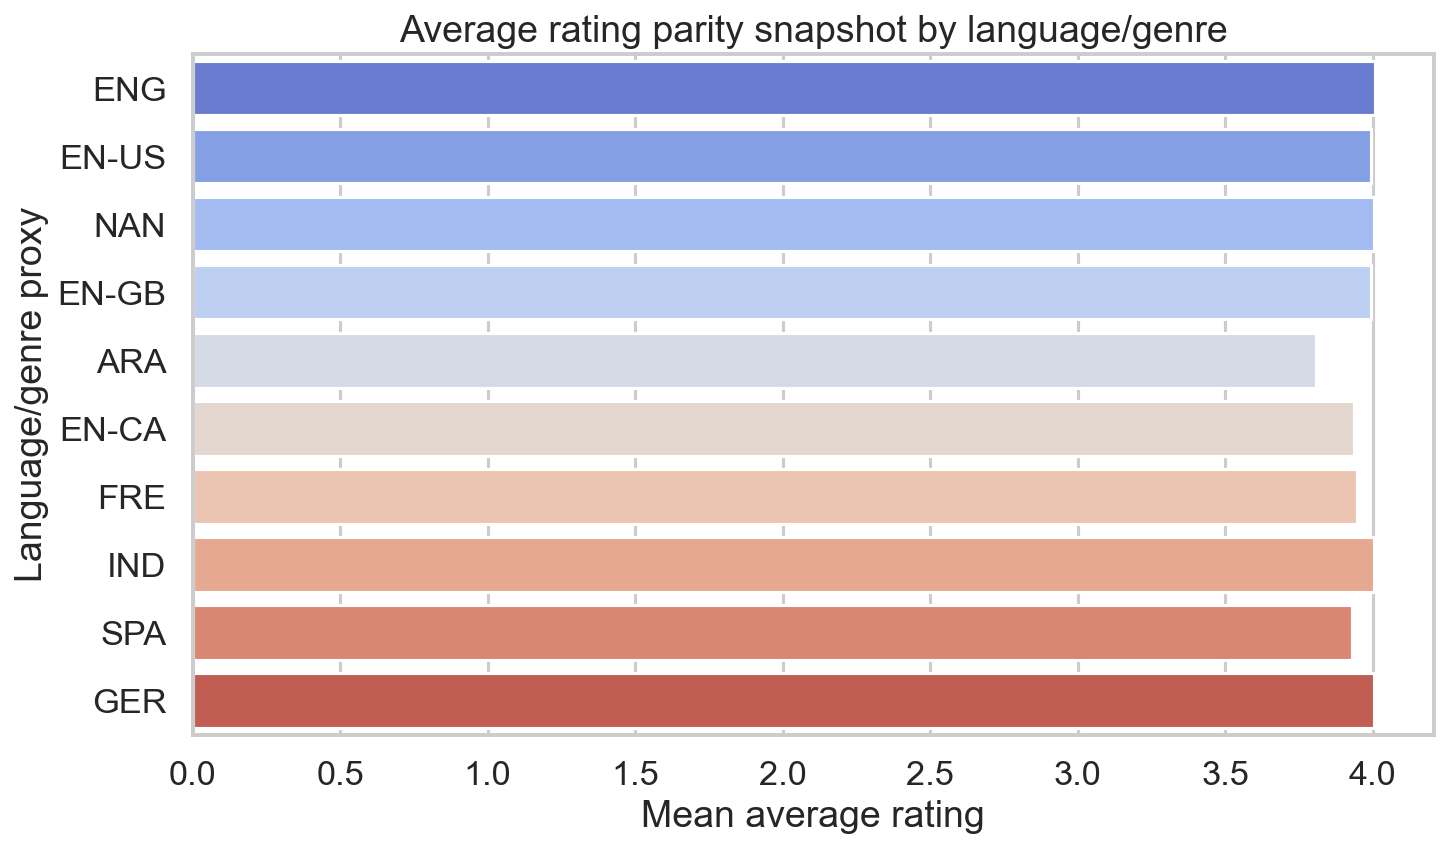
\includegraphics[width=.8\linewidth]{parity_language_bar.png}}{\begin{center}\textit{parity\_language\_bar.png was unavailable at build time.}\end{center}}
    \caption{Relative NDCG@10 performance across language cohorts.}
    \label{fig:parity-fig}
\end{figure}

\parityStatusNote
